% !TEX root = main.tex

We present the results of the LCA analysis in relation to the 1) embodied  emissions, 2) a calculation of the emission factor, 3) sensitivity of the LCA to design and location, and 4) a comparison to other PV technologies.

\subsection{LCA of the Adaptive Solar Facade Manufacture}

A breakdown of six major midpoint impact indicators based of the ReCiPe methodology \cite{goedkoop2009recipe}  can be found in Figure  \ref{fig:embodied}. The largest embodied GWP contribution in the ASF comes from the solar panels, followed by the electronics and the supporting structure. The control and electronics systems play a large role in freshwater eutrophication, and human toxicity due to the high life cycle emissions of electronic systems.



\begin{figure}[H]
\begin{center}
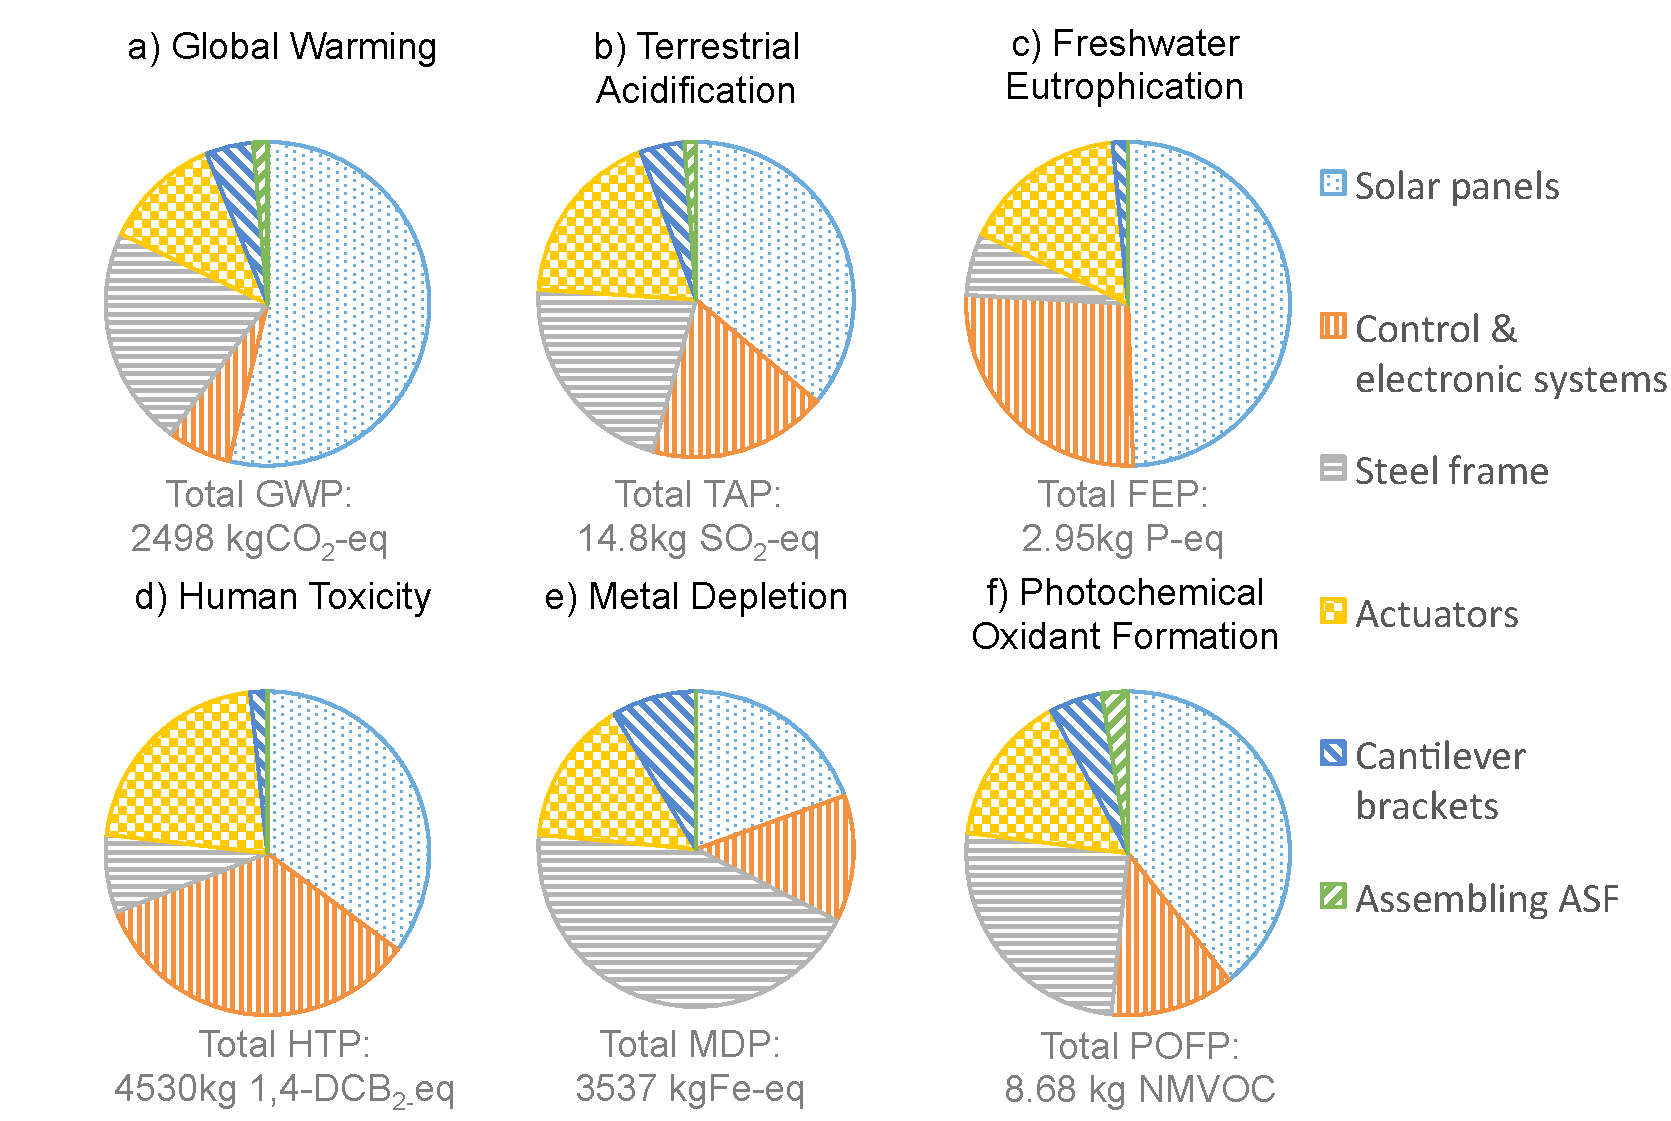
\includegraphics[width=\textwidth, trim= 0cm 0cm 0cm 0cm,clip]{pieembodied}
\caption{Embodied emission breakdown of six major midpoint indicators. The solar panels, control/electronics, and steel frame have the highest life cycle impact}
\label{fig:embodied}
\end{center}
\end{figure}

\subsection{Calculation of GWP Emission Factor}
The combined GWP of main inputs to the ASF, previously described in Figure \ref{fig:BOS}, can be illustrated using a waterfall chart as shown in Figure \ref{fig:waterfall}. 


This gives us a final emission of 3037kgCO$_2$-eq. When we include the energy savings through adaptive shading in our system expansion, the final emissions come down to -8318kgCO$_2$-eq. Dividing these values by the photovoltaic electricty production over a 20 year life time of 9175kWh, we get an emission factor of 331gCO$_2$-eq/kWh for the system without adaptive shading and -906 gCO$_2$-eq/kWh with adaptive shading.


\begin{figure}[H]
\begin{center}
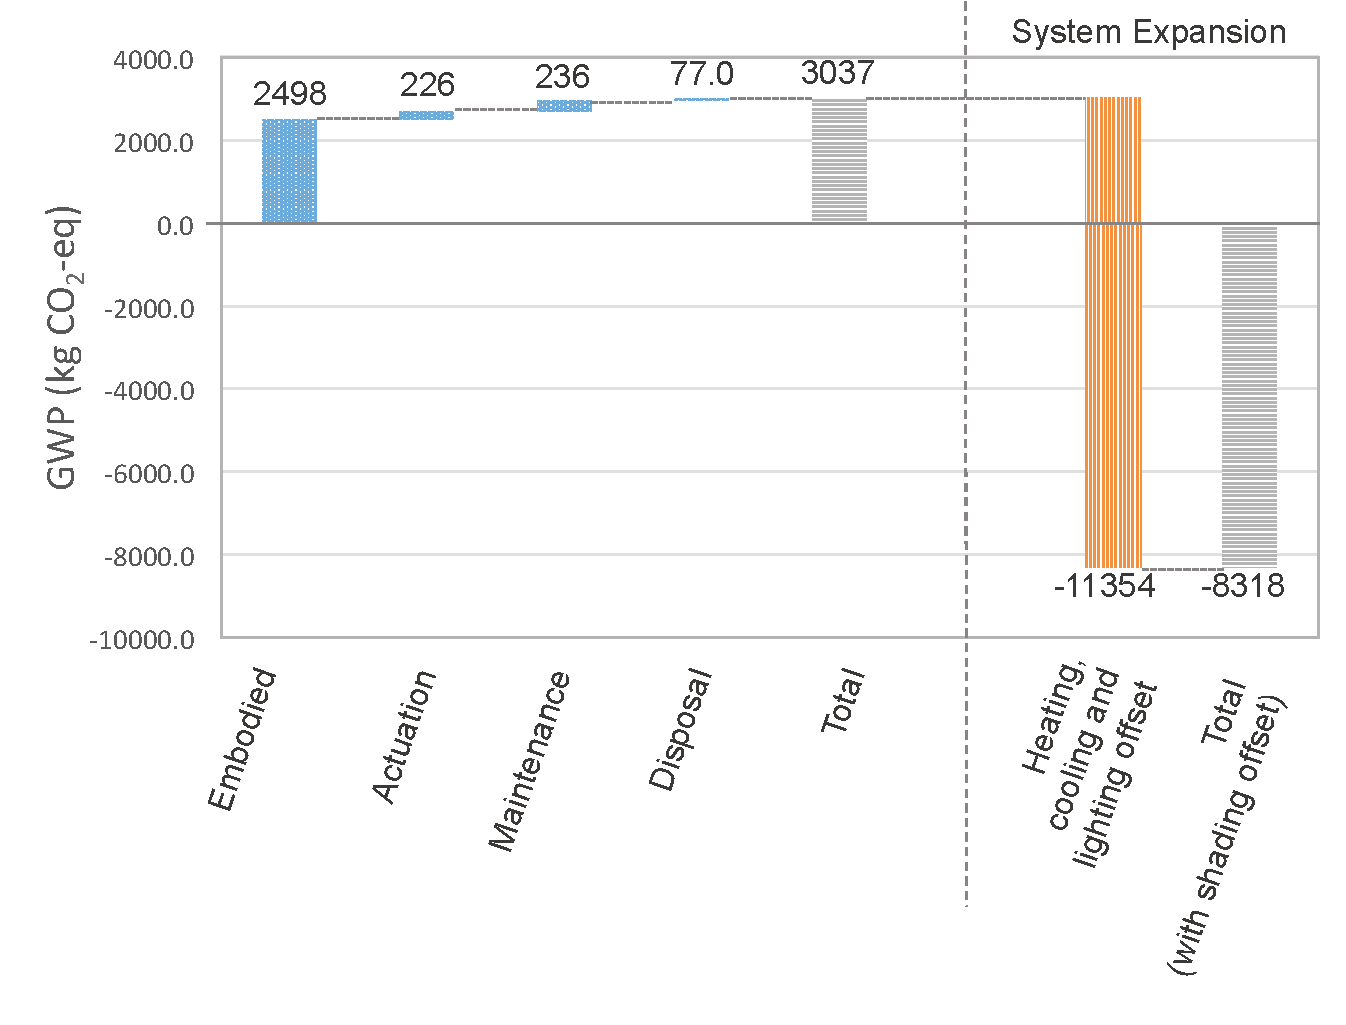
\includegraphics[width=\textwidth, trim= 0cm 0cm 0cm 0cm,clip]{waterfall}
\caption{Waterfall diagram of GWP of the ASF not including photovoltaic electricity production. When reading from left to right, the far left bar details the embodied carbon emissions. The second, third and fourth bar detail the actuation, maintenance, and disposal respectively. This leaves us with our final emissions value (grey bar) of 3037kgCO$_2$-eq. The orange bar details the emission reduction through adaptive shading which is part of our system expansion bringing the total down to -8318kgCO$_2$-eq. When we divide these totals by the photovoltaic electricity production (9174kWh) we gain an emission factor of 331gCO$_2$-eq/kWh for the system without adaptive shading and -906 gCO$_2$-eq/kWh with adaptive shading. Note that the waterfall chart itself doesn't show PV electricity generation. This is taken into account in the emission factor.}

\label{fig:waterfall}
\end{center}
\end{figure}



\subsection{Sensitivity Analysis}


The sensitivity analysis is shown in Figure \ref{fig:sens}. The performance of the ASF is dependent on the location where it is operated as explained in Section \ref{ch:Meth:Opp}. Changing the weather files of the simulation, and the electricity mix of the country brings interesting results. Geneva has a similar climate to Frankfurt, however the local electricity mix is dominated by hydro and nuclear power which has a very low GWP potential \cite{itten2012life}. This would then increase the emission factor of the ASF to 53.5 gCO$_{2}$-eq/kWh. This difference arises as the greenhouse gas emission savings of adaptive shading are dependent on the emission factor of the grid mix.
Spain on the other hand has a warmer climate, with higher solar radiation, but a less greenhouse gas intensive electricity mix. This ultimately results in a similar emission factor of the ASF of -825 gCO$_{2}$-eq/kWh.\\


We also present a case where we remove the actuators and necessary control system for a dynamic system. Instead, we have panels that are optimally orientated at 45$^{\circ}$ to the horizontal axis. This reduces embodied greenhouse gas emissions by 12.1\% from the baseline highlighted in Figure \ref{fig:embodied}. However the reduction in electricity production, and savings through adaptive shading, result in a 15\% higher emission factor.\\

The choice of actuator has a small impact on the embodied carbon emissions. Changing a single Soft Robotic Actuator (including the air compressor, tubing, and maintenance) to a classical servo motor increases the total embodied GWP by 23\% from 2498 kg CO$_{2}$-eq to 3073 kg CO$_{2}$-eq. However, the servo motors have lower operational emissions and maintenance. Ultimately an ASF with servo motors has a 1.5\% higher emission factor. \\


The control system design should be carefully thought out due to the high embodied human toxicity, freshwater eutrophication and terrestrial acidification. However simplifying the actuation control electronics has a minimal effect as the majority of the emissions lie in the inverter, cables, and air compressor. In terms of GWP, there is a 0.3\% difference which is negligible.



\begin{figure}[H]
\begin{center}
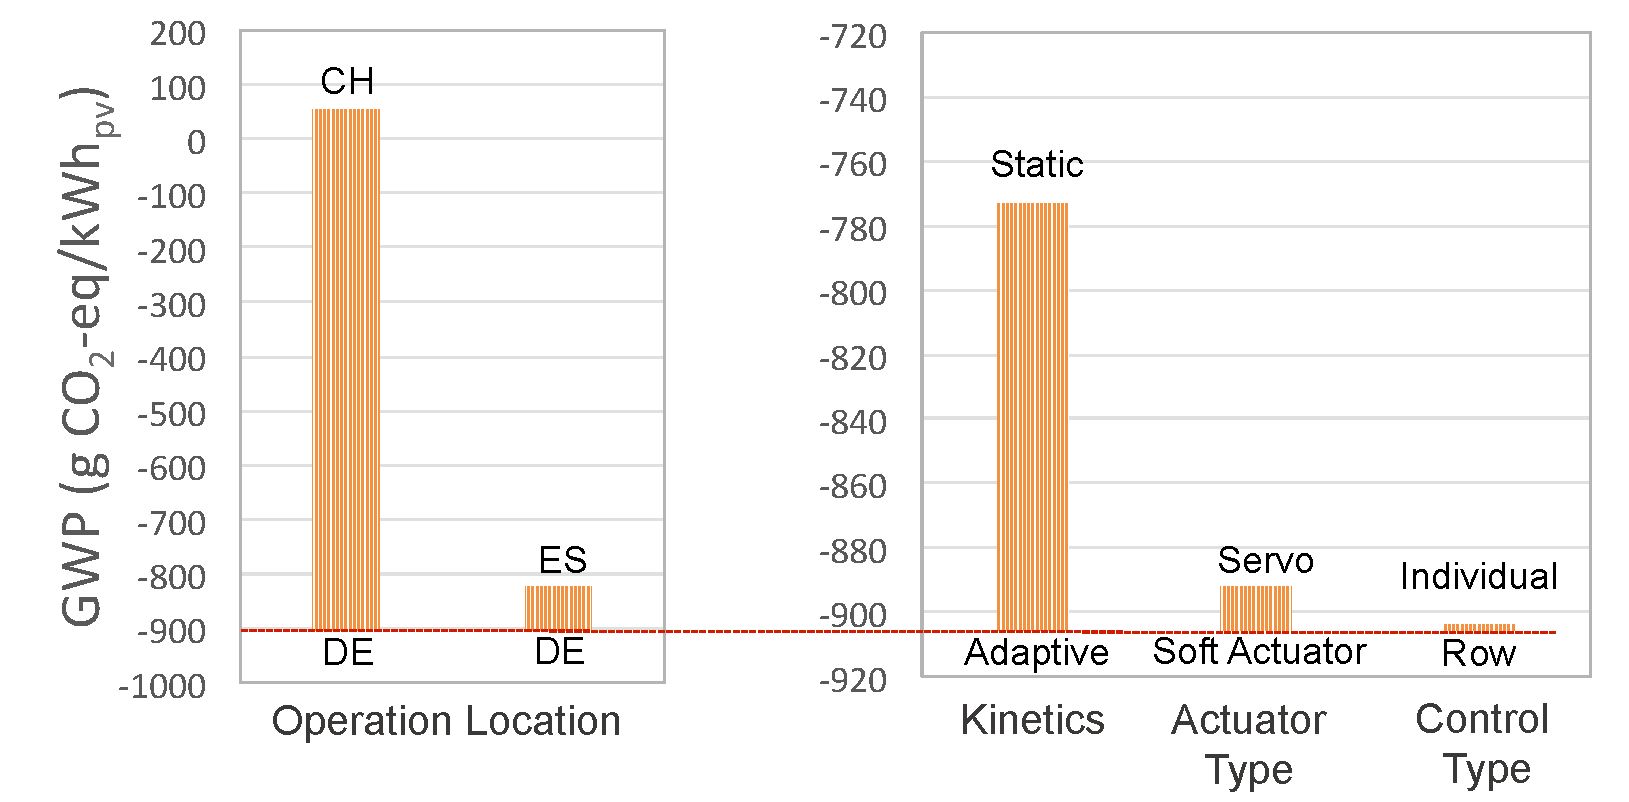
\includegraphics[width=\textwidth, trim= 0cm 0cm 0cm 0cm,clip]{sens.pdf}
\caption{Sensitivity analysis of the emission factor including the HVAC impact of adaptive shading based on location, actuation system, and control system}
\label{fig:sens}
\end{center}
\end{figure}

\subsection{Comparison to existing PV technologies}

Comparison of the ASF to other PV technologies and the German electricity mix is highlighted in Figure \ref{fig:compPV}. This comparison is conducted in Frankfurt am Main with an average irradiation of 855 kWh/m$^2$/year.\

The blue bars detail systems with no added shading benefits. Here we present the ASF, a static optimally orientated facade as used in Figure \ref{fig:sens}, and three classical flat facade installations.  
The orange bars detail the system expansion where the ASF is built over glazed surfaces which also bring energy savings to the building. Because the GWP savings through adaptive shading offsets the entire embodied GWP, we have a system with a negative emission factor.





\begin{figure}[H]
\begin{center}
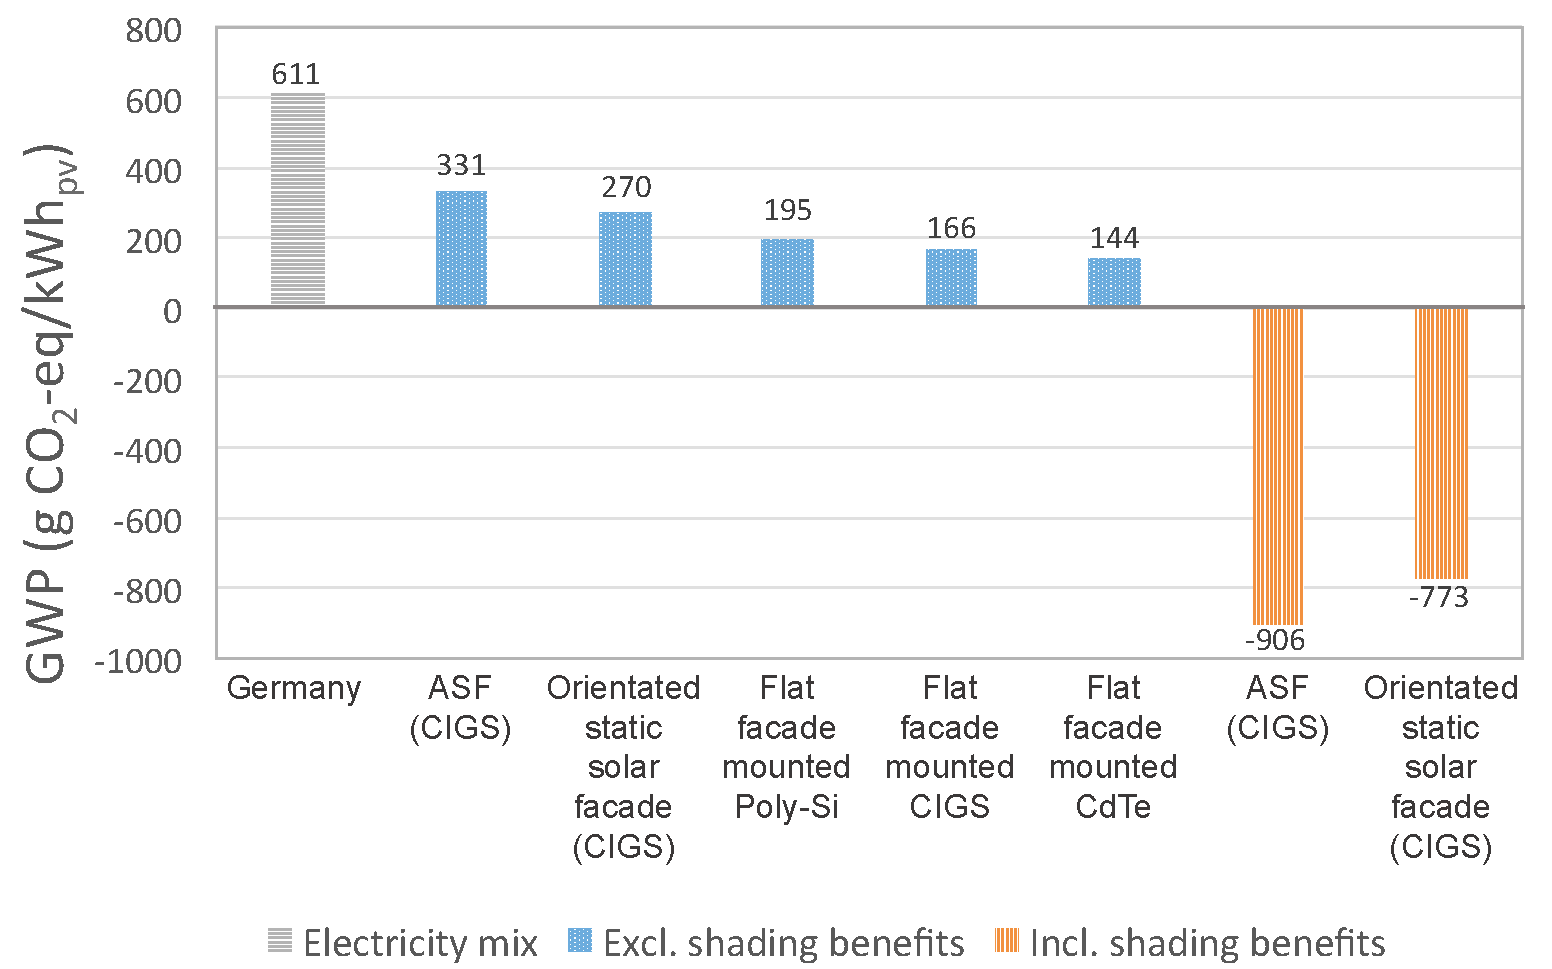
\includegraphics[width=\textwidth, trim= 0cm 0cm 0cm 0cm,clip]{compPV.pdf}
\caption{Comparison of facade installations in Germany with an average facade irradiation of 855kWh/m$^2$/year.
We compare an ASF to an optimally orientated static facade, and classic flat facade mounted PV solutions. The orange bars include the system expansion of energy savings through adaptive shading.}
\label{fig:compPV}
\end{center}
\end{figure}

